\documentclass[conference]{IEEEtran}
\usepackage[T1]{fontenc}
\usepackage{cite}
\usepackage{amsmath,amssymb,amsfonts}
\usepackage{graphicx}
\usepackage{booktabs}
\usepackage{url}
% Replace these fields after the author information is confirmed.
\newcommand{\AuthorName}{Author Name}
\newcommand{\AuthorDepartment}{Department or School}
\newcommand{\AuthorInstitution}{University or Institution}
\newcommand{\AuthorLocation}{City, Country}
\newcommand{\AuthorEmail}{Email to be confirmed}

\graphicspath{{figures/}}

\begin{document}

\title{Text-Side Low-Rank Adaptation of CLIP for Flickr30k Retrieval}
\author{\IEEEauthorblockN{\AuthorName}
\IEEEauthorblockA{\textit{\AuthorDepartment}\\
\textit{\AuthorInstitution}\\
\AuthorLocation\\
\AuthorEmail}}
\maketitle

\begin{abstract}
Adapting CLIP for image--text retrieval requires separating the benefit of attention updates from that of training the output projection. A small trainable parameter count also need not preserve inference speed. We compare zero-shot CLIP, projection-only adaptation, and manually implemented text-side low-rank adaptation (LoRA) with the projection, while freezing the visual branch. Experiments use a fixed Flickr30k annotation split and three paired training seeds. Evaluation ranks all 1,000 test images against all 5,000 captions. LoRA plus projection achieves $89.21\pm0.11$ percent mean recall, compared with $87.82\pm0.14$ for projection-only training and 84.13 for zero-shot CLIP. The paired improvement over projection-only training is 1.39 percentage points. The adapted model updates 458,752 parameters, approximately 0.303 percent of its total. However, its unmerged implementation increases single-text encoding latency from 7.77 to 9.73 milliseconds on a Tesla T4. Query-level transitions and real retrieval failures show that aggregate improvements coexist with regressed matches and ambiguous correspondence labels. These findings support text-side attention adaptation within the tested budget, while distinguishing parameter efficiency from runtime efficiency.
\end{abstract}

\begin{IEEEkeywords}
image--text retrieval, CLIP, low-rank adaptation, parameter-efficient fine-tuning, Flickr30k
\end{IEEEkeywords}

\section{Introduction}
Image--text retrieval ranks photographs from a natural-language description and, in the reverse direction, ranks descriptions from an image. Both directions require distinguishing a corresponding example from other candidates depicting similar objects, actions, or scenes. This distinction makes retrieval quality depend on the candidate gallery and the definition of a positive match.

Contrastive Language--Image Pre-training (CLIP) aligns images and text in a shared embedding space and supports zero-shot transfer~\cite{radford2021clip}. Its pretrained representations offer a strong baseline, but their usefulness does not determine the most effective adaptation scope under a limited training budget. When the visual branch remains frozen, a trainable text projection can already alter cross-modal alignment. Attention adaptation therefore needs a stronger comparator than the original checkpoint alone.

Low-rank adaptation (LoRA) adds compact trainable weight updates while retaining pretrained weights~\cite{hu2022lora}. This reduces the number of updated parameters, but an unmerged implementation introduces additional inference operations. Retrieval quality, trainable parameters, and measured latency consequently answer different practical questions.

This project asks whether text attention adaptation adds retrieval value beyond projection-only training, and what runtime cost accompanies that gain. We compare three adaptation scopes from the same CLIP ViT-B/32 checkpoint on a fixed Flickr30k annotation split. Paired sampling plans, validation-based checkpoint selection, and complete candidate galleries control the principal experimental variables. The contribution is a manual implementation and controlled evaluation of established methods, rather than a new architecture or adaptation algorithm. Real successes, failures, and regressed queries define the scope of the conclusions.

\section{Related Work}
\subsection{Visual--Semantic Retrieval}
Learning a common space for visual and linguistic representations is a longstanding approach to retrieval. Karpathy and Fei-Fei study visual--semantic alignment using images and descriptions~\cite{karpathy2015alignments}. VSE++ emphasizes hard negatives when learning retrieval embeddings~\cite{faghri2018vse}. These studies motivate attention to the candidate gallery and to closely related negatives. Our experiments use a pretrained contrastive model and a symmetric cross-entropy objective; they do not implement either earlier retrieval architecture.

\subsection{Pretrained Vision--Language Representations}
CLIP uses paired image and text supervision to align the modalities~\cite{radford2021clip}. Its ViT-based visual encoder belongs to the image-patch Transformer family~\cite{dosovitskiy2021vit}. We retain its visual features and ask whether a limited change to the text branch improves retrieval on the supplied Flickr30k split. External leaderboard numbers are not used as baselines because checkpoint pretraining, gallery composition, and split conventions can differ.

\subsection{Parameter-Efficient Adaptation}
Adapter methods update compact added modules while retaining pretrained parameters~\cite{houlsby2019adapters}. LoRA instead parameterizes a weight update using two low-rank matrices~\cite{hu2022lora}. We apply this construction to text attention and compare it with projection-only adaptation. The experiments use a manual implementation, not a library-provided PEFT wrapper. Our rank is fixed at eight; neither the strategy comparison nor the parameter-count plot is a rank ablation.

\section{Dataset and Data Integrity}
\subsection{Resources and Actual Experimental Scale}
Flickr30k provides real photographs with human-written descriptions~\cite{young2014flickr}. Its source portal permits non-commercial research and educational use while retaining the original image copyright and terms~\cite{flickrportal}. The image archive prepared for this project contains 31,783 JPEG files. The supplied JSON annotation, obtained from a Karpathy-format annotation mirror~\cite{karpathymirror}, references 31,014 distinct images and 155,070 captions. We use exactly these referenced images. The remaining 769 image files are not assigned to any experimental split or added as extra training examples.

\begin{table}[t]
\caption{Actual annotation-defined partitions. Caption counts describe available annotations; training uses one caption per image in each epoch.}
\label{tab:data}
\centering
\begin{tabular}{lrr}
\toprule
Partition & Images & Available captions\\
\midrule
Train & 29,000 & 145,000\\
Validation & 1,014 & 5,070\\
Test & 1,000 & 5,000\\
\midrule
Total & 31,014 & 155,070\\
\bottomrule
\end{tabular}
\end{table}

Table~\ref{tab:data} reports the counts read from the actual file, rather than replacing them with a conventional benchmark count. The supplied JSON's existing \texttt{split} field defines the partitions. It is not regenerated randomly. Image IDs and filenames are both unique within the annotation and disjoint across train, validation, and test. Each image and all five captions remain in one partition. The code uses the recorded filename to locate an image; an annotation image ID is not assumed to be its JPEG basename.

\subsection{Validation and Preprocessing}
Preflight checks matched all referenced filenames and fully decoded their images without errors. Empty captions, repeated IDs, repeated filenames, and split intersections were checked before training. These checks establish isolation of the supplied annotations; they do not establish absence of visually similar scenes or overlap with the original CLIP pretraining corpus.

Images are converted to RGB and processed by the checkpoint's original PIL-based CLIP processor, including deterministic resizing, center cropping to $224\times224$, and normalization. Captions use the corresponding tokenizer, with truncation at 77 tokens. Training and timing experiments pad text to length 77. Retrieval evaluation pads each feature-extraction batch to its longest sequence, up to the same limit. All five captions are retained during evaluation.

Images, annotations, model weights, and processor files are supplied as local Kaggle inputs. Hashes identify the annotation, base checkpoint, and sampling plans. The Kaggle experiments operate offline, avoiding dependence on a live model or dataset download service during execution.

\section{Method}
\subsection{Embedding Model and Adaptation Strategies}
Let $x_i$ be an image and $t_j$ a caption. The encoders and their projections produce normalized vectors
\begin{align}
\mathbf v_i &= \frac{P_v f_v(x_i)}{\|P_v f_v(x_i)\|_2},\\
\mathbf u_j &= \frac{P_t f_t(t_j)}{\|P_t f_t(t_j)\|_2}.
\end{align}
Both vectors have 512 dimensions, and cosine similarity is $s_{ij}=\mathbf v_i^\top\mathbf u_j$. The implementation projects each encoder's pooled output into the shared retrieval space. Figure~\ref{fig:method} shows the main adaptation strategy.

\begin{figure*}[t]
\centering
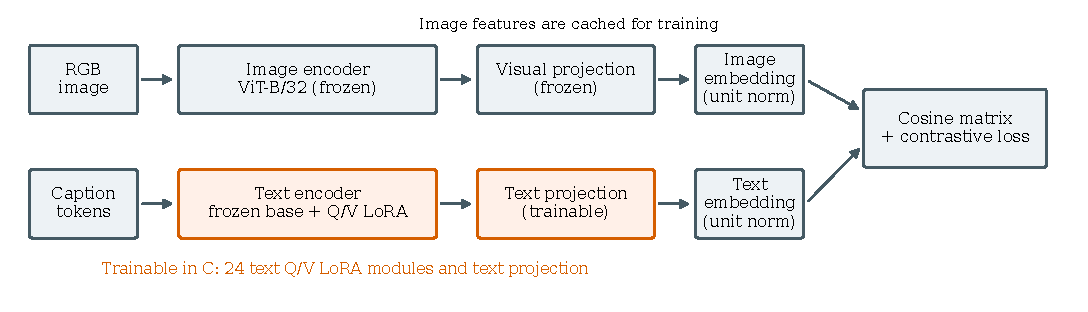
\includegraphics[width=\textwidth]{method.pdf}
\caption{Main strategy C. The visual encoder and visual projection remain frozen. Original text weights remain frozen, while low-rank branches in text query/value projections and the text projection are trainable. Normalized image features are cached for training. The diagram describes the implemented computation; it is not a generated experimental result.}
\label{fig:method}
\end{figure*}

\textit{A: Zero-shot CLIP.} The original pretrained model is evaluated without any parameter update.

\textit{B: Projection-only.} Both encoders and the visual projection remain frozen. Only the bias-free $512\times512$ text projection is updated, giving 262,144 trainable parameters.

\textit{C: LoRA plus projection.} The text projection is updated as in B. In addition, query and value linear modules in each of the 12 text Transformer blocks receive low-rank branches. This produces 24 adapted modules. Queries determine attention compatibility with keys, while values carry the information aggregated by attention. Keys, attention output projections, embeddings, normalization layers, original query/value weights and biases, and the remaining pretrained parameters stay frozen. All strategies start from the same original checkpoint. C does not start from a trained B checkpoint.

\subsection{Manual Low-Rank Layers}
For a frozen linear weight $W_0\in\mathbb R^{d_{\rm out}\times d_{\rm in}}$, the implemented layer computes
\begin{equation}
 h(\mathbf z)=W_0\mathbf z+\mathbf b_0+
 \frac{\alpha}{r}BA\mathbf z,
\label{eq:lora}
\end{equation}
where $A\in\mathbb R^{r\times d_{\rm in}}$ and $B\in\mathbb R^{d_{\rm out}\times r}$. This follows the low-rank update construction of LoRA~\cite{hu2022lora}. We set $r=8$ and $\alpha=8$, so the scale is one. $A$ is initialized using Kaiming uniform initialization and $B$ to zero. The initial added branch is therefore zero. There is no LoRA dropout, and the branches remain unmerged for all reported measurements.

With text width 512, the added parameter count is
\begin{equation}
 24\,r(512+512)=196{,}608.
\end{equation}
Including the text projection gives 458,752 trainable parameters. The original model has 151,277,313 parameters, while the unmerged adapted model has 151,473,921. Thus, C updates 0.3029\% of its total parameters. A preflight optimizer-step check verifies zero-initialization equivalence, updates to the trainable matrices, and unchanged frozen-parameter snapshots. The initial zero $B$ also explains why $A$ need not have a nonzero gradient on the first step.

\subsection{Caption Sampling and Contrastive Objective}
Expanding every image into five independent pairs can place repeated images in one batch. A diagonal-only contrastive target would then treat another caption of that same image as a negative. We avoid this known source of incorrect negatives by indexing training examples by image. Each epoch visits every training image once and chooses one of its five captions. There are 29,000 pairs per epoch, not 145,000 simultaneously expanded training pairs.

For each seed, a saved plan specifies both the image permutation and the caption choice for each image at each epoch. B and C share this plan. Each batch therefore has distinct image IDs, with one positive pair per row and column. This removes duplicate-image negatives; it does not guarantee that descriptions of different images are semantically unrelated.

For a batch of size $b$, the logits are $\ell_{ij}=\beta s_{ij}$, where $\beta$ is the exponential of CLIP's frozen logit-scale parameter. The loss is
\begin{align}
\mathcal L_{\mathrm{I2T}} &=-\frac1b\sum_{i=1}^{b}
 \log\frac{\exp(\ell_{ii})}{\sum_{j=1}^{b}\exp(\ell_{ij})},\\
\mathcal L_{\mathrm{T2I}} &=-\frac1b\sum_{i=1}^{b}
 \log\frac{\exp(\ell_{ii})}{\sum_{j=1}^{b}\exp(\ell_{ji})},\\
\mathcal L &=\tfrac12(\mathcal L_{\mathrm{I2T}}+\mathcal L_{\mathrm{T2I}}).
\end{align}
Gradients update only the designated text parameters. The complete visual branch is frozen, so deterministic normalized image features are precomputed in FP32 and reused across epochs. Text features are recomputed during training so C can backpropagate through its low-rank branches.

\section{Experiments}
\subsection{Setup and Fair Comparisons}
Experiments use one Tesla T4 on Kaggle, with approximately 14.56 GiB of GPU memory. All computation uses a single GPU. The recorded environment uses Python 3.13.15, PyTorch 2.11.0+cu128~\cite{paszke2019pytorch}, and Transformers 5.16.1~\cite{wolf2020transformers}. Other dependencies are torchvision 0.26.0+cu128, huggingface\_hub 1.29.0, and Pillow 13.0.0.

B and C use five epochs, batch size 64, AdamW~\cite{loshchilov2019adamw}, learning rate $10^{-5}$, weight decay 0.01, gradient norm clipping at 1.0, and no learning-rate scheduler. Each epoch has 454 updates, including the final batch of eight images. The text encoder and projection forward pass use FP16 autocast; normalized features, logits, and cross-entropy are computed in FP32. Gradient scaling starts at 1024. All 30 recorded training epochs have zero skipped optimizer updates. Validation and final retrieval evaluation use FP32.

We train B and C with seeds 42, 43, and 44. Within each seed, the data, base checkpoint, sample order, caption choices, optimizer settings, precision, and epoch budget are identical. The two principal contrasts are A versus C for overall adaptation and B versus C for the added contribution of attention adaptation. These are fixed-budget comparisons, not separately optimized hyperparameter searches for each method.

After every epoch, the full validation gallery is evaluated. Each run retains the trained epoch with the highest validation mR; all six runs select epoch five. The final test set is used only after checkpoint selection and configuration locking. We report all three seeds, rather than choosing the seed with the highest test score. Qualitative examples use seed42, fixed before inspecting which seed is best on the test set.

\subsection{Full-Gallery Retrieval Metrics}
Feature extraction is batched for memory efficiency, but metrics are computed after assembling the complete gallery. For $N=1000$ test images, I2T has $N$ queries and $5N$ caption candidates; T2I has $5N$ queries and $N$ distinct image candidates. A single FP32 similarity matrix has shape $1000\times5000$.

Let $g(j)$ map caption $j$ to its image. I2T uses
\begin{equation}
 r_i^{\mathrm{I2T}}=\min_{j:g(j)=i}\operatorname{rank}_{i}(j),
\end{equation}
so any of the five positive captions can satisfy a hit. T2I uses the rank of the single image $g(j)$. Ranks are one-based, with candidate-index order resolving tied scores. For a query set $Q$,
\begin{equation}
 R@K=\frac{100}{|Q|}\sum_{q\in Q}\mathbf{1}[r_q\leq K].
\end{equation}
MedianRank is the ordinary median of these query ranks, including averaging the two middle ranks for an even count. Mean recall, mR, averages the six directional Recall values, giving the two directions equal weight rather than pooling their different query counts. Unit checks cover multi-positive minimum rank, mapping permutations, Recall boundaries, and the even-count median.

\begin{table*}[t]
\caption{Final test retrieval. Recall and mR are percentages. B/C report means $\pm$ sample standard deviations across three training seeds. A is evaluated once without adaptation. MedianRank is 1 for every reported run.}
\label{tab:main}
\centering
\footnotesize
\setlength{\tabcolsep}{3pt}
\begin{tabular}{lrrrrrrrrr}
\toprule
& \multicolumn{4}{c}{Image-to-text} & \multicolumn{4}{c}{Text-to-image} & \\
\cmidrule(lr){2-5}\cmidrule(lr){6-9}
Method & R@1 & R@5 & R@10 & MedR & R@1 & R@5 & R@10 & MedR & mR\\
\midrule
% BEGIN GENERATED ROWS
A: Zero-shot & 79.30 & 95.00 & 98.10 & 1 & 58.84 & 83.44 & 90.08 & 1 & 84.13 \\
B: Projection-only & $81.10 \pm 0.52$ & $96.53 \pm 0.15$ & $99.03 \pm 0.21$ & 1 & $66.91 \pm 0.13$ & $89.29 \pm 0.14$ & $94.04 \pm 0.03$ & 1 & $87.82 \pm 0.14$ \\
C: LoRA + projection & $84.17 \pm 0.46$ & $97.53 \pm 0.15$ & $99.40 \pm 0.10$ & 1 & $68.87 \pm 0.27$ & $90.40 \pm 0.02$ & $94.87 \pm 0.10$ & 1 & $89.21 \pm 0.11$ \\
% END GENERATED ROWS
\bottomrule
\end{tabular}

\end{table*}

\subsection{Attention Adaptation Adds Value Beyond the Projection}
Table~\ref{tab:main} shows that both supervised adaptations improve on the original checkpoint. B raises mR from 84.13 to 87.82, a 3.69-point gain. C reaches $89.21\pm0.11$, a 5.08-point gain over A. Thus, the projection baseline accounts for a substantial part of the overall improvement, while adding LoRA provides a further gain under matched conditions.

Relative to B, C improves I2T R@1 by 3.07 points and T2I R@1 by 1.95 points. These lower-rank hits benefit more visibly than already high I2T R@10, which increases from 99.03 to 99.40. Different positive-set sizes also matter: I2T has five annotated positives per query whereas T2I has one. Their absolute Recall values should not be interpreted as identical tests of encoder quality.

\begin{table}[t]
\caption{Paired final-test mR by training seed. Differences are percentage points. All selected epochs are five.}
\label{tab:paired}
\centering
\begin{tabular}{rrrr}
\toprule
Seed & B & C & C$-$B\\
\midrule
% BEGIN GENERATED ROWS
42 & 87.72 & 89.19 & +1.47 \\
43 & 87.98 & 89.32 & +1.34 \\
44 & 87.76 & 89.10 & +1.35 \\
% END GENERATED ROWS
\bottomrule
\end{tabular}

\end{table}

The C-minus-B mR difference is positive for every seed (Table~\ref{tab:paired}), with a paired mean and sample standard deviation of $1.3878\pm0.0741$ points. This consistency supports the observed additional benefit within the tested configuration. Three seeds do not establish statistical significance or robustness to other datasets, learning rates, or ranks. The uncertainty reported here is training-seed variation, not a confidence interval over independently sampled test queries.

All MedianRank values equal one because more than half the queries retrieve an annotated positive at the first position. This metric consequently hides improvements and failures in the remaining ranks. It is retained for protocol completeness and interpreted jointly with Recall.

\begin{figure*}[t]
\centering
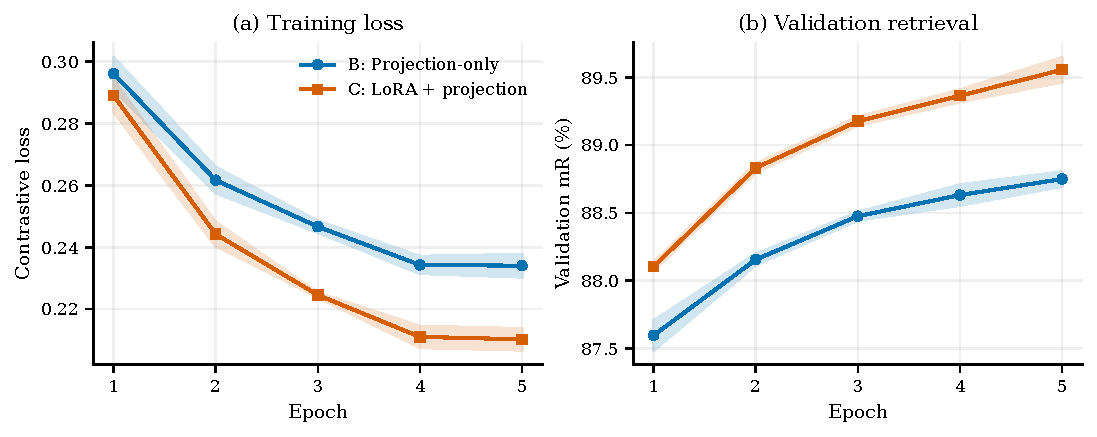
\includegraphics[width=\textwidth]{training_validation.pdf}
\caption{Training loss and full-validation mR over five epochs. Curves show means across seeds42/43/44; shaded regions are sample standard deviations, with no smoothing. The panels have different y-axis scales.}
\label{fig:curves}
\end{figure*}

\subsection{Optimization and Validation Behavior}
Figure~\ref{fig:curves} shows decreasing mean training loss for both trainable strategies. C reaches lower mean loss and higher validation mR within the same five-epoch budget. Caption resampling changes batch difficulty between epochs, so individual runs need not have monotonically decreasing loss. Validation mR is $88.7497\pm0.0542$ for B and $89.5551\pm0.0908$ for C, compared with 84.5036 for A. The paired validation mR gain is $0.8054\pm0.0366$ percentage points.

These validation values are checkpoint-selection measurements, not substitutes for final test performance. Because the best observed epoch is the final budgeted epoch, the experiment does not establish that either strategy has fully converged.

\subsection{Trainable Parameters and Measured Costs}
Table~\ref{tab:compute} separates trainable parameters from the complete model. B changes existing weights and therefore has the same total parameter count and inference operation structure as A. C adds 196,608 low-rank parameters. Its small trainable fraction does not imply that the original encoders disappear from the forward pass.

\begin{table*}[t]
\caption{Model complexity and recorded training cost. Major-operator counts use one $224\times224$ image and one 77-token text, with 1 MAC = 2 FLOPs. Pair GFLOPs sums both encoders. Training seconds are averaged over the 15 epochs per strategy; peak is the largest PyTorch allocated-memory peak. Cache preparation and validation time are excluded from epoch training time.}
\label{tab:compute}
\centering
\footnotesize
\setlength{\tabcolsep}{4pt}
\begin{tabular}{lrrrrrrrr}
\toprule
Group & Total (M) & Trainable (K) & Trainable (\%) & Image GMACs & Text GMACs & Pair GFLOPs & Epoch (s) & Peak (GiB)\\
\midrule
% BEGIN GENERATED ROWS
A & 151.277 & 0.000 & 0.0000 & 4.4088 & 2.9798 & 14.7772 & -- & -- \\
B & 151.277 & 262.144 & 0.1733 & 4.4088 & 2.9798 & 14.7772 & 20.25 & 0.696 \\
C & 151.474 & 458.752 & 0.3029 & 4.4088 & 2.9949 & 14.8074 & 48.91 & 1.791 \\
% END GENERATED ROWS
\bottomrule
\end{tabular}

\end{table*}

The counting code measures convolution and linear modules with hooks and explicitly includes the two attention matrix products and the manual low-rank branches. Attention is counted as dense computation over the complete sequence, including masked positions. Bias and residual additions, normalization, activation, Softmax, embedding lookup, low-rank scaling, and gallery scoring/ranking are excluded. These values are theoretical major-operator counts, not complete hardware instruction counts.

At length 77, the low-rank additions cost 15,138,816 MACs: about 0.51\% of baseline text encoding. Image encoding remains 4.4088 GMACs in all groups. Total image-plus-text encoding increases by about 0.20\% in C. Projection-only training costs about 20.25 seconds per cached-image epoch, versus 48.91 seconds for C. Allocated-memory peaks are approximately 0.696 and 1.791 GiB. C needs gradients through intermediate text activations even though the original weights are frozen; trainable-parameter count alone therefore does not determine training memory or speed.

\subsection{Encoding Speed and Cached Matching}
We separately measure online encoding operations and cached matching. Inputs are resident on \texttt{cuda:0}, models are in evaluation mode, and precision is FP32 with unmerged LoRA. Batch-one latency uses 20 warm-up calls followed by 100 synchronized wall-clock samples. It includes Python dispatch and completion synchronization. Batch32 throughput uses ten warm-up calls and five rounds of ten consecutive forwards, synchronizing at round boundaries.

\begin{figure*}[t]
\centering
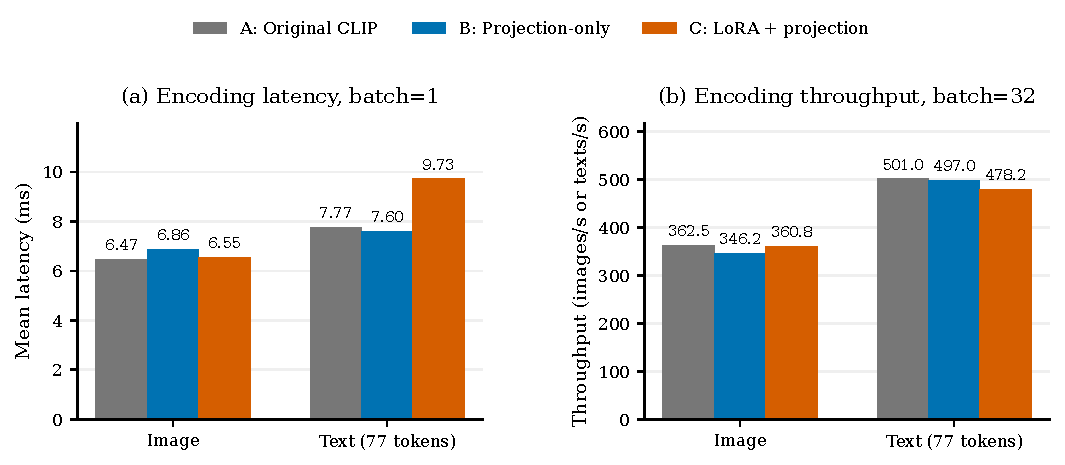
\includegraphics[width=\textwidth]{speed.pdf}
\caption{Single-T4 FP32 encoding measurements using seed42 checkpoints. The image/text inputs are shared across groups. Batch-one bars are repeated-call mean latencies; batch32 bars are measured throughput. These are not three-training-seed averages. Read/decode, preprocessing, tokenization, and host/device transfer are outside timing.}
\label{fig:speed}
\end{figure*}

Figure~\ref{fig:speed} shows 6.55 ms per image and 9.73 ms per 77-token text for C. The original model takes 6.47 and 7.77 ms, respectively. Recorded p95 latencies are retained in the project report and source CSV. C's single-text latency is about 25.3\% higher, despite the small counted-MAC increase. Batch32 text throughput falls from 500.98 to 478.20 texts/s, about 4.5\%, while C processes 360.80 images/s. Variations between the identical A/B visual branches should be treated as measurement variation, not evidence of architectural acceleration.

\begin{table}[t]
\caption{Cached single-query similarity plus sorted Top-5 latency (ms), using 1,000 image candidates or 5,000 caption candidates.}
\label{tab:cached}
\centering
\begin{tabular}{lrr}
\toprule
Group & T2I & I2T\\
\midrule
% BEGIN GENERATED ROWS
A & 0.0668 & 0.1058 \\
B & 0.0695 & 0.1103 \\
C & 0.0736 & 0.1064 \\
% END GENERATED ROWS
\bottomrule
\end{tabular}

\end{table}

Cached retrieval uses 20 warm-up calls and 200 synchronized samples, rotating through 64 already encoded queries. Each query scores the full candidate gallery and applies sorted Top-5 selection. C takes about 0.074 ms for T2I and 0.106 ms for I2T (Table~\ref{tab:cached}). These are matching latencies with both query and gallery features precomputed. They are not end-to-end request times: a new request also requires input preparation, encoding, transfers, and result presentation. The timing operator selects Top-5; metric evaluation separately computes complete stable rankings.

\subsection{Successful Retrievals and Residual Failures}
The qualitative procedure uses a fixed seed of 2026 to select examples within predefined categories: both models correct at Top-1, C correcting an A Top-1 miss, and a C Top-5 miss. Selection is based on the saved rank arrays, and plotted ranks are checked against the final evaluation. Figures~\ref{fig:t2i} and~\ref{fig:i2t} compactly show the improvement and failure categories for the predefined seed42 model. Complete baseline and adapted Top-5 displays remain in the notebook and artifact package.

\begin{figure*}[t]
\centering
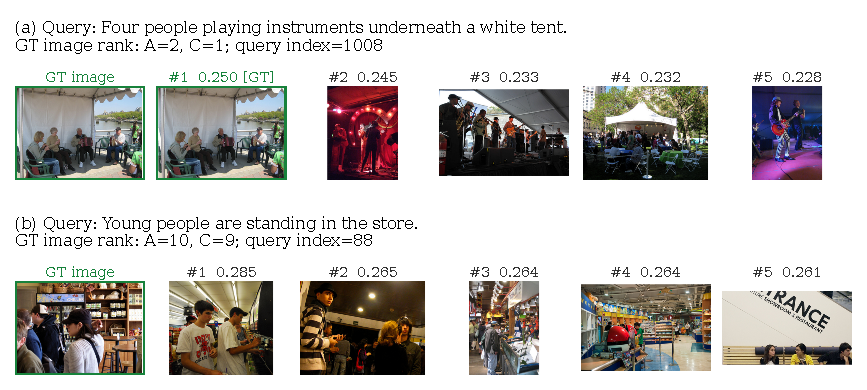
\includegraphics[width=\textwidth]{qualitative_t2i.pdf}
\caption{Text-to-image examples: the supplied ground-truth image and C's Top-5 candidates with cosine scores. (a) Instrument-playing query: A ranks the positive second, C first. (b) Store query: the positive moves from rank10 to rank9, remaining outside Top-5. GT denotes the dataset correspondence; other images may still be semantically relevant. All images and scores come from real saved examples.}
\label{fig:t2i}
\end{figure*}

For T2I, ``Four people playing instruments underneath a white tent'' moves its corresponding image from rank two to rank one after adaptation. This illustrates a local ordering correction rather than recovery of a completely unrelated scene. In contrast, ``Young people are standing in the store'' remains difficult: its correct image improves from rank ten to nine. Several returned candidates contain people in shops or similar indoor settings. Other annotations of the positive image mention a cap, a gray sweater, waiting in line, and a coffee shop, but these details are absent from the selected query. The example is consistent with insufficient textual specificity for instance-level discrimination.

\begin{figure*}[t]
\centering
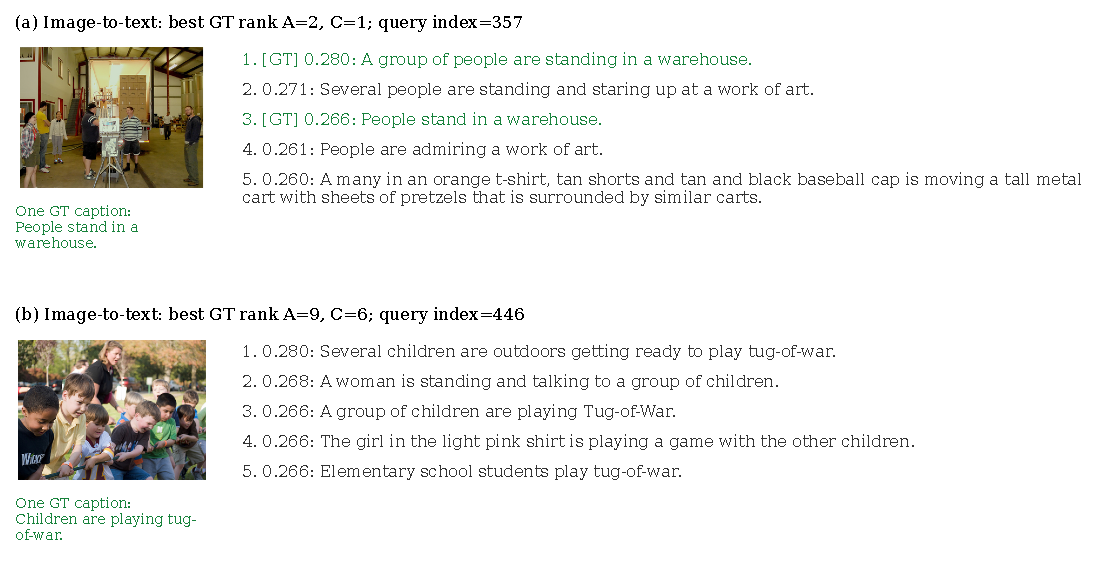
\includegraphics[width=\textwidth]{qualitative_i2t.pdf}
\caption{Image-to-text examples with C's actual Top-5 captions and cosine scores. (a) The warehouse image improves from best positive rank2 to rank1. (b) The tug-of-war image improves from rank9 to rank6. A GT tag indicates membership in the query image's five annotated captions, not a general judgment of semantic truth. One short positive caption is shown beside each image for context.}
\label{fig:i2t}
\end{figure*}

For I2T, the warehouse example promotes a corresponding description to first place. The tug-of-war failure is more subtle. Its correct annotations include ``Children are playing tug-of-war,'' while a returned non-corresponding caption says ``A group of children are playing Tug-of-War.'' The query image visibly contains children pulling a rope. Thus, the model retrieves the activity theme, but the exact annotation-based positive set is not reached within five candidates. Some returned captions are broadly compatible with the scene even though they belong to another image. This illustrates a limitation of treating correspondence labels as exhaustive semantic relevance judgments; it does not justify changing the benchmark labels after evaluation.

\begin{table}[t]
\caption{Top-1 query transitions from A to C at fixed seed42, counted from saved ranks. ``Only'' identifies which model retrieves an annotated positive.}
\label{tab:transitions}
\centering
\footnotesize
\setlength{\tabcolsep}{4pt}
\begin{tabular}{lrrrr}
\toprule
Direction & Both & A only & C only & Neither\\
\midrule
% BEGIN GENERATED ROWS
I2T & 750 & 43 & 89 & 118 \\
T2I & 2785 & 157 & 673 & 1385 \\
% END GENERATED ROWS
\bottomrule
\end{tabular}

\end{table}

To complement selected images, Table~\ref{tab:transitions} audits every query at seed42. C corrects 89 I2T Top-1 misses but loses 43 previous hits; for T2I it corrects 673 and loses 157. The net gains explain the higher aggregate Recall without suggesting uniform improvement. T2I captions share images and are not independent observations, so these counts are descriptive and are not used for a per-caption significance test. Cosine magnitudes also change after adaptation: a lower absolute score does not imply a worse within-model ranking.

\section{Discussion and Reproducibility}
\subsection{Interpreting the Quality--Cost Trade-off}
The strategy comparison separates two sources of adaptation benefit. Updating the text projection already improves alignment, while Q/V adaptation provides additional flexibility under the same budget. This supports attention adaptation in the tested setting without establishing superiority over full text tuning, other adaptation methods, or independently optimized projection training. CLIP and LoRA remain the methodological foundations~\cite{radford2021clip,hu2022lora}; the project contributes implementation and controlled evidence.

The runtime findings qualify the parameter-efficiency result. Small low-rank projections add limited arithmetic but can introduce execution overhead when left unmerged. Their operations and dispatch costs are a plausible explanation for the latency gap, although individual kernels were not profiled. Direct measurements of merged and unmerged implementations would test whether that penalty persists after deployment-oriented changes.

\subsection{Code, Evidence, and Restored Results}
The submission provides \path{CLIP_Flickr30k_code_package_20261030.zip}, with captured experiments, a fresh-training entry, and a restore/report entry. The accompanying availability manifest identifies their exact relative paths and records SHA256 values for the code and experimental-artifact archives. The code package includes key notebook outputs; the artifact archive preserves checkpoint deltas, paired sampling plans, histories, metrics, query ranks, and timing details. These records complement the manuscript's source-data files.

A later Kaggle session restored 76 files with matching hashes and loaded all six checkpoints. Every C\_seed42 validation metric reproduced its saved value, with maximum absolute difference zero. Subsequent reporting read existing final-test and timing records without rerunning those measurements. Historical summaries are labeled as recovered records. The manuscript's verification script checks saved-data arithmetic and document consistency; this is distinct from running model inference.

\subsection{Boundaries and Discriminating Next Tests}
The gain is conditional on one checkpoint, one supplied split, three seeds, rank eight, and five epochs. A matched rank sweep and a longer validation-selected budget would test whether it persists across capacity and convergence conditions. No rank-four or rank-sixteen result is claimed.

Image-level isolation does not exclude visual near-duplicates or overlap with original CLIP pretraining. Additional datasets and larger galleries would test transportability beyond the 1,000-image test gallery. Multi-positive training could expose more captions while handling repeated-image positives, although semantically related negatives would remain. Full-request timing would also determine the contribution of preprocessing and transfer costs excluded here.

\section{Conclusion}
Text-side adaptation improved CLIP retrieval on the supplied Flickr30k split, and manual Q/V LoRA added a consistent gain beyond projection-only training. The main configuration achieved $89.21\pm0.11$ test mR while updating 458,752 parameters. Its unmerged branches nevertheless increased text encoding latency, and some previously correct queries regressed. The practical conclusion is conditional: assess attention adaptation against a trained projection baseline, and measure runtime independently of parameter count.

\clearpage
\raggedbottom
\IEEEtriggeratref{7}
\bibliographystyle{IEEEtran}
\bibliography{references}
\end{document}
